\documentclass{standalone}
\usepackage{pgfplots}
\pgfplotsset{compat=newest}

\begin{document}
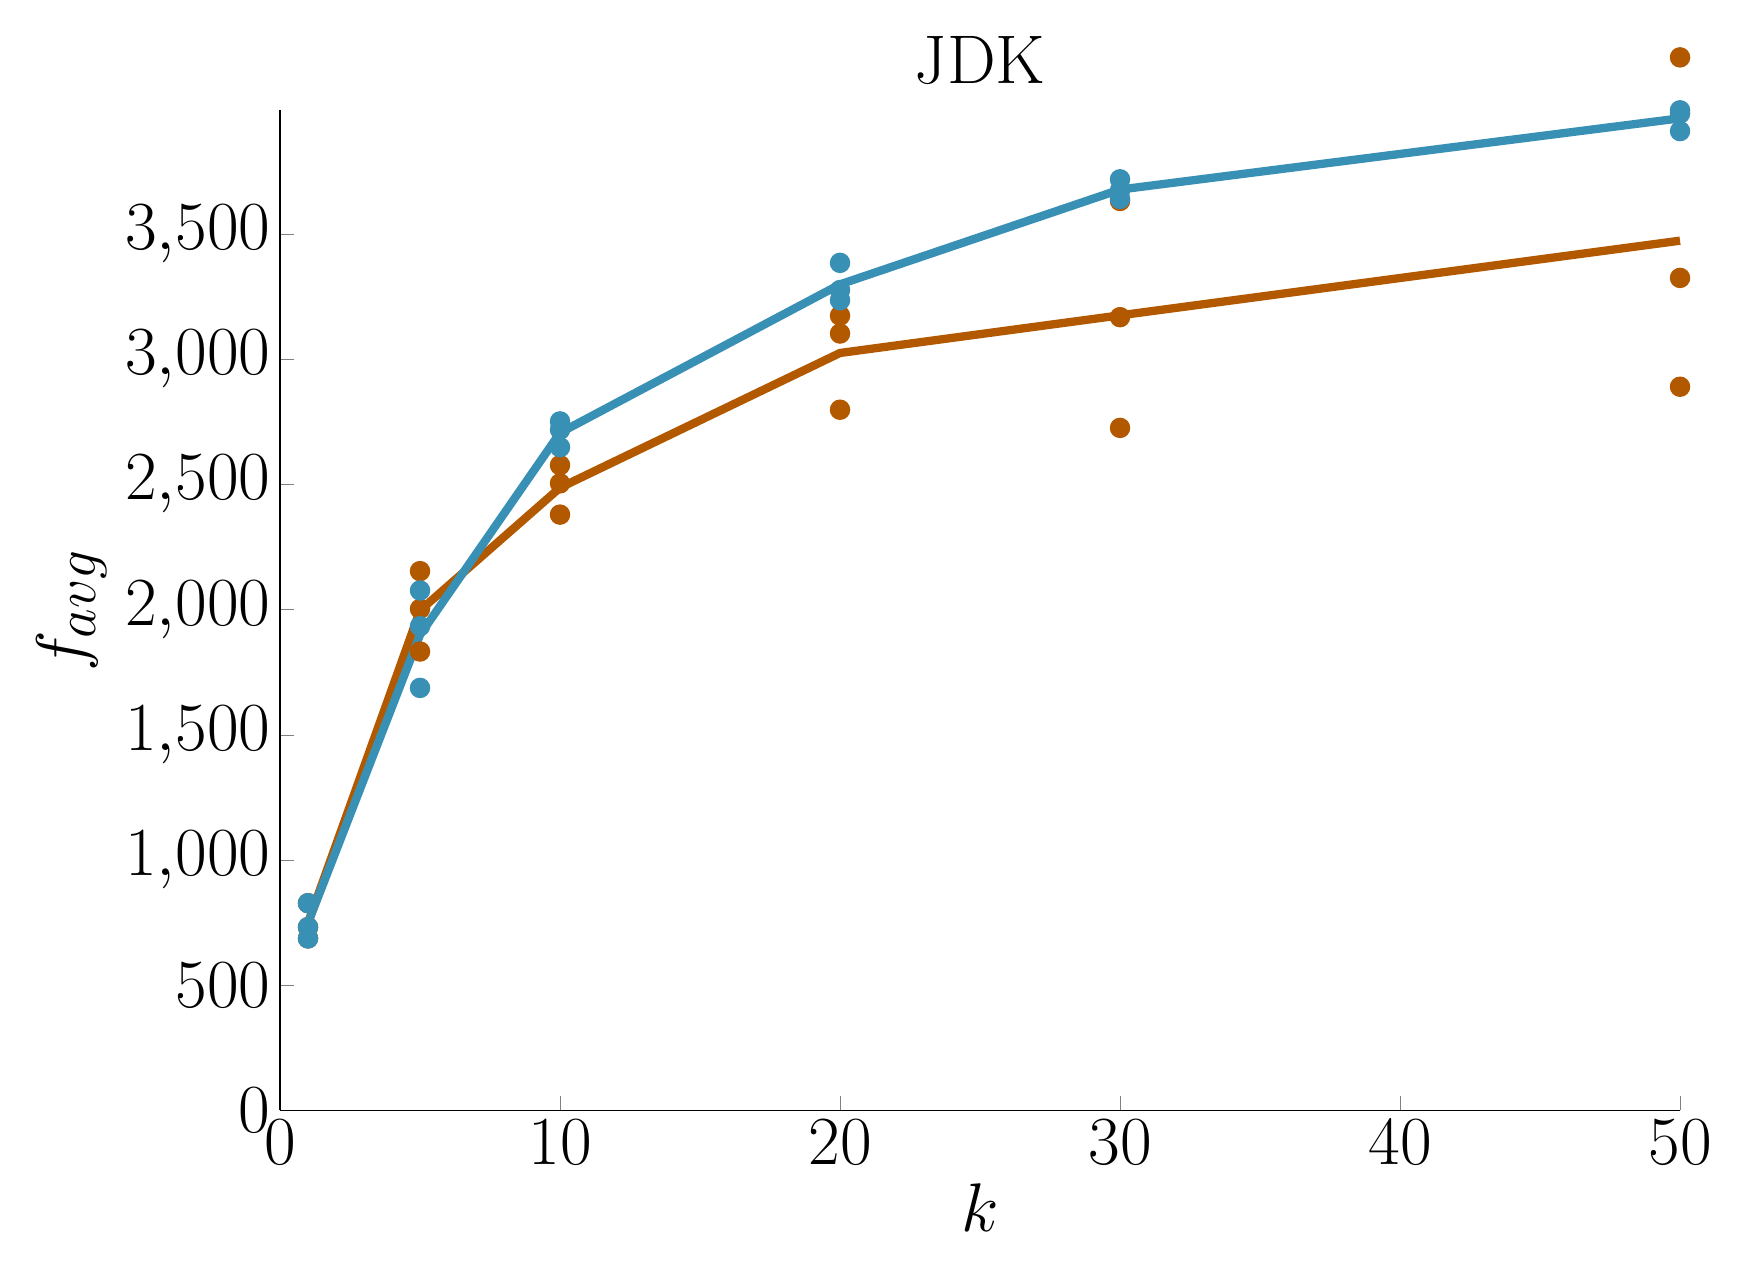
\begin{tikzpicture}

\begin{axis}[%
title style={font=\Huge},
title=JDK,
tick label style={font=\Huge},
label style={font=\Huge},
legend style={font=\Huge},
view={0}{90},
max space between ticks=50pt,
width=7in,
height=5in,
scale only axis,
xmin=0, xmax=50,
xtick={0, 10, 20, 30, 40, 50},
xlabel={$k$},
ymin=0, ymax=3994.45,
%ytick={0, 200, 400, 600, 800, 1000},
ylabel={$f_{avg}$},
major tick length=5pt,
axis lines*=left,
legend cell align=left,
clip=false]

\addplot [
only marks,
mark=*,
mark size=3.5pt,
color=orange!70!black,
%solid,
%line width=2pt,
]
coordinates{
(1,686.6)(1,731.65)(1,827.45)(5,1832.7)(5,2002.9)(5,2153.85)(10,2379.5)(10,2504.45)(10,2577.0)(20,2798.4)(20,3102.85)(20,3174.15)(30,2725.85)(30,3168.15)(30,3632.35)(50,2890.25)(50,3324.95)(50,4205.85)
};

\addplot [
only marks,
mark=*,
mark size=3.5pt,
color=cyan!70!black,
%solid,
%line width=2pt,
]
coordinates{
(1,686.6)(1,731.65)(1,827.45)(5,1687.25)(5,1933.65)(5,2076.45)(10,2648.6)(10,2718.5)(10,2751.8)(20,3235.75)(20,3276.65)(20,3385.0)(30,3640.45)(30,3674.65)(30,3718.85)(50,3911.45)(50,3981.3)(50,3994.45)
};

\addplot [
color=orange!70!black,
solid,
line width=3pt
]
coordinates{
(1,748.566666667)(5,1996.48333333)(10,2486.98333333)(20,3025.13333333)(30,3175.45)(50,3473.68333333)
};

\addplot [
color=cyan!70!black,
solid,
line width=3pt
]
coordinates{
(1,748.566666667)(5,1899.11666667)(10,2706.3)(20,3299.13333333)(30,3677.98333333)(50,3962.4)
};


\end{axis}
\end{tikzpicture}
\end{document}
